\subsection{Pong Soup}
\label{sec_pong}

The first evaluation domain is a set of synthetic variants of the
Atari game of Pong ("Pong Soup") where the visuals and gameplay have been
altered, thus providing a setting where we can be confident that there
are transferable aspects of the tasks.  The variants are
\emph{Noisy} (frozen Gaussian noise is added to the inputs);
\emph{Black} (black background); \emph{White} (white
background); \emph{Zoom} (input is scaled by 75\% and
translated); \emph{V-flip, H-flip, and VH-flip} (input is
horizontally and/or vertically flipped). Example frames are shown in
Fig. \ref{fig:datasets}.
The results of training two columns on the Pong variants, including
all relevant baselines are shown in Figure
\ref{pong_results}. Transfer scores are summarized over all target
tasks in Table~\ref{table:main}.

\begin{figure}[h]
  \centering
    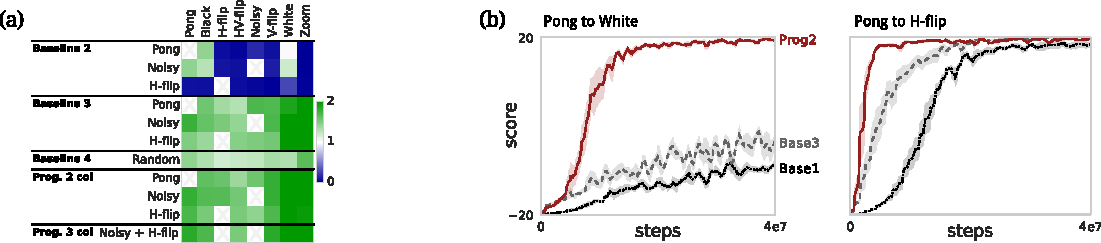
\includegraphics[width=1.\textwidth]{figures/transfer_pong.pdf}
    \caption{(a) Transfer matrix. Colours indicate transfer scores (clipped at 2).
      For progressive nets, the first column is trained on Pong, Noisy,
      or H-flip (table rows); the second column is trained on each of the
      other pong variants (table columns). (b) Example learning curves.}
    \label{fig:atari_results}
    \label{pong_results}
\end{figure}

We can make
several observations from these results. Baseline 2 (single column, only output layer is finetuned; see Fig.~\ref{fig:baselines})
fails to learn the target task in most
experiments and thus has negative transfer. This approach is quite standard
in supervised learning settings, where features from
ImageNet-trained nets are routinely repurposed for new domains.
As expected, we observe high positive transfer with baseline 3 (single column, full finetuning),
a well established paradigm for transfer.
Progressive networks outperform this baseline however in terms of both median and mean score, with
the difference being more pronounced for the latter. As the mean is
more sensitive to outliers, this suggests that progressive networks are better
able to exploit transfer when transfer is possible (i.e. when source and target domains are compatible). Fig.~\ref{pong_results}~(b) lends
weight to this hypothesis, where progressive networks are shown to significantly
outperform the baselines for particular game pairs.
Progressive nets also compare
favourably to baseline 4,
confirming that progressive nets are indeed taking
advantage of the features learned in previous columns.

\textbf{Detailed analysis}

\begin{figure}[h]
  \centering
    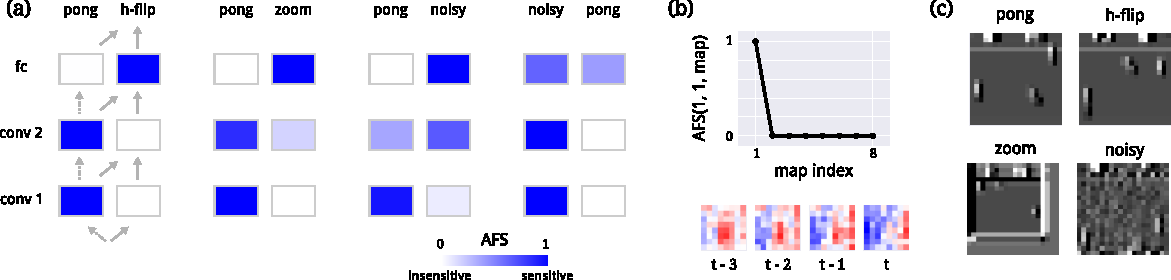
\includegraphics[width=.95\textwidth]{figures/pong_results_neil.pdf}
    \caption{(a) Transfer analysis for 2-column nets on Pong variants.
      The relative sensitivity of the network's outputs on the columns
      within each layer (the AFS) is indicated by the darkness of shading.
      (b) AFS values for the 8 feature maps of
      conv. 1 of a 1-column Pong net. Only one feature map is
      effectively used by the net; the same map is also used by the
      2-column versions. Below: spatial filter components (red =
      positive, blue = negative). (c) Activation maps of the filter in (b) from example
      states of the four games.}
    \label{fig:pong_results_neil}
\end{figure}

We use the metric derived in Sec.~\ref{sec_transfer} to
analyse what features are being transferred between Pong variants.
We see that when switching from Pong to H-Flip, the network reuses the
same components of low and mid-level vision (the outputs of the two
convolutional layers; Figure \ref{fig:pong_results_neil}a). However, the fully connected layer must be
largely re-learned, as the policy relevant features of the task (the
relative locations/velocities of the paddle and ball) are now in a new
location. When switching from Pong to Zoom, on the other hand,
low-level vision is reused for the new task, but new mid-level vision
features are learned. Interestingly, only one low-level feature appears
to be reused:
(see Fig.~\ref{fig:pong_results_neil}b): this is a spatio-temporal
filter with a considerable temporal DC component. This appears
sufficient for detecting both ball motion and paddle position in the
original, flipped, and zoomed Pongs.

Finally, when switching from Pong to Noisy, some new low-level
vision is relearned. This is likely because the first layer
filter learned on the clean task is not sufficiently
tolerant to the added noise. In contrast, this problem does not apply
when moving from Noisy to Pong (Figure
\ref{fig:pong_results_neil}a, rightmost column), where all of vision
transfers to the new task.
